\chapter{Preguntas tecnicas Angular}
\section{Diferencias entre la compilacion JIT vs AOT}
JIT : Va hacer mas rapido ,sin embargo poco perforrmance time.\\
AOT Compilation : Tomas mas tiempo en compilar ,es mas performante,mas liviano.Tiene check de template
(Esta verificacion no esta en JIT).
\begin{figure}[H]
	\centering
	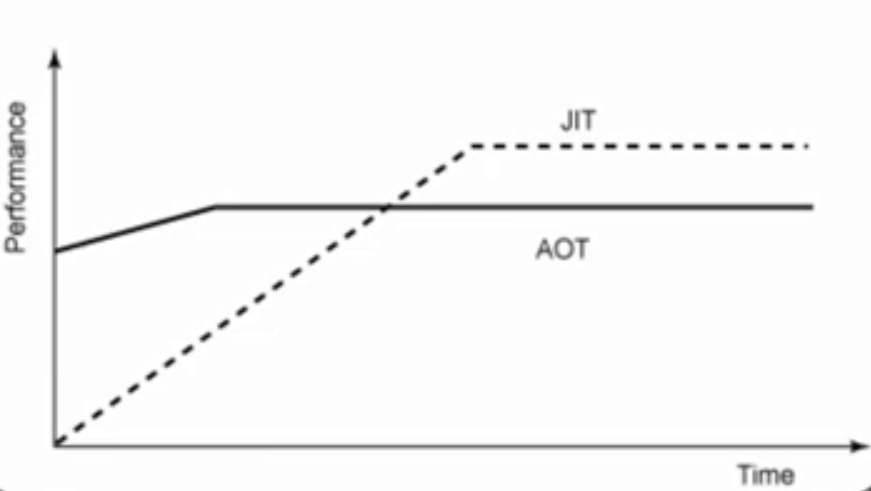
\includegraphics[scale=0.3]{images/fig_3_1.jpg}
	\caption{JIT vs AOT.}
\end{figure}
\section{Que es un modulo y cuales son sus partes}
Un modulo representa una funcionalidad de la aplicacion .Contiene todo lo necesaro y solo lo necesario .
Un modulo va a declarar componentes,provaiders (Servicios),
entry components(Models),mportar otros modulos,shared modulos.
\section{Ciclo de vida de un componente}
ng OnChanges() : Se ejecuta antes del ngOnInit().Lo hace debido a cambios.\\
ng OnInit() : Se inicializa los atributos , se instancia el componente.\\
ng AfterViewInit() : Se renderiza la vista y todos sus hijos.\\
ng OnDestroy() : Se utiliza cuando queremos liberar memoria.
\section{Que es lazy loading de modulos}
Es carga perezosa , se carga las cosas a medida que vamos necesiitandolo.\\
Mejora la perrformance .Tener en memoria 
solo lo que vamos a usar.
\section{Diferencia entre observable y promesa}
Una promesa es que en alguna instancia de tiempo , algo va a suceder.Y esto va ocurrir una vez.\\
En cambio un observable , varias veces , puede o no resolverrse.\\
Nota : Una promesa es un observable.
\section{Comunicar informacion entre componentes no relacionales}
Servicios,problemas de async.\\
Input/Outputs , problemas de jerarquia y contaminacion (Hijo-Padre-Hijo).\\
Observables , forma correcta .
\section{View Child vs Content Child}
View Child :Busca en el template.\\
Content Child :Busca dentro del ng Content.
\section{HTTP interceptor}
Es un servicio , que se utiliza como un middleware de peticiones.\\
Ejemplo : Spinner.
\section{Que es una directiva y que tipos hay}
Aumento de funcionalidad de elementos del DOM.\\
Estructura * (ngFor,ngIf).\\
Attributes [{}] (input,ng class,events,ouput,data bamding).
\section{Que es un pipe}
Son funciones que transforman expresiones en el template.Toma datos como entrada y los
transforman en una salida deseada.
\section{Que resulta de un ng build}
Tree Shaking : Se elimina lo que no se usa para tener el bundle final.\\
Uglifying : Se genera el resultado final para que no pueda ser leido el codigo.\\
Minification : Reduce todo a una sola linea.Reduce la cantidad de peso de los archivos.\\
Bundling : Se genera un bundle de la app.\\
Production Mode : Saca cualquier cosa que se usa en desarrollo.Para tenerlo lo mas performante
posible.
\section{Optimizar la performance de angular}
Lazy loading.\\
Minimizar bundles.\\
Production Mode.\\
Buenas practicas.\\
Optimizacion de imagenes.\\
Modo Strict.
\section{Que son los custom pipes}
Podemos crear nuestros propios pipes.Un pipe es una clase decorada con metadatos de pipe @Decorador,
que importa desde la angular core. 
\section{PIPE puro e impuro diferencias}
Puro solo se llama cuando se detecta un cambio en el valor.\\
Impuro se llama cuando cada ciclo de deteccion de cambio (Sin importar si el valor a cambiado).
\section{Que es HttpClient}
Es un API HTTP de cliente simplificada conocida como httpClient que se basa en XMLHttpRequest.\\
Esta libreria esta en @angular/common/http.
\section{Como se realiza el manejo de errores}
Se debe manejar el error pensando el objeto de error como segundo parameto en la llamada de el
metodo SubScribe().
\section{Que son los componentes dinamicos}
Son componentes que su ubicacion no esta definida en el momento de la compilacion.El componente se
instancia en la aplicacion en tiempo de ejecucion.
\section{Cuales son los distintos tipos de diectivas}
Componentes : Son directivas con plantillas.\\
Estructurales : Cambian el dise\~no del DOM al agregar o eliminar atributos.\\
Atributos : Cambian la apariencia o el comportamiento de un elemento , componente u otra directiva.
\section{Como se crean directivas con CLI}
CLI ng generate directiva creara una clase de tipo directiva.\\
Esto creara el archivo fuente y el archivo de testing (.spec,.ts) y declara la directiva en el modulo raiz.
\section{Cuales son los diferentes tipos de compilacion en angular}
Ofrece 2 formas de compilar : JIT (Just-in-time) y AOT (Ahead-of-time).
\section{Que es angular}
Es un framework de codigo abierto basado en typescript .Plantillas declarativas,inyeccion de dependencias y otras
caracteristicas que facilitan el desarrollo.
\section{Que son las directivas}
A\~naden comporrtamiento a un elememto del DOM ya existente.
\section{Que es un componente}
Controla una parte de la pantalla llamada vista.Son bloques de construccion de inteface de usuario.
\section{Angular CLI}
Es una interfaz de linea de comandos para montar y construir aplicaciones de angular.
\section{Diferencia entre constructor y ngOnInit}
El constructor se ejecuta primeo,despues ngOnInit.El constructo se utiliza con fines de inicializacion, mientras que ngOnInit es especifico de angular, se usa para definir el banding.
\section{Algunas directivas estructurales}
ngIf,ngFor.
\section{Directiva *ngIf}
Inserta o elimina elementos del DOM basados en una condicion true o false.
\section{Que es la intepolacion}
Es una sintaxis especial de angular, perrmite hacer el banding de una propiedad{{}}.